\section{METHODS} \label{section:methods}
We have staged our optimization process into three distinct phases.  The following subsections describe these phases.

\subsection{Phase-1:}
This phase's primary goal is to express the BPMax equation in \alphaz\ , perform the first-level optimization on the most compute-intensive portion of the task and get a baseline estimation.

\paragraph{Multi-dimensional Affine Schedule for Double Max-plus Operation}
We simplify the BPMax computation based on the following recurrence equation as the very first step.
\begin{equation}
\label{eqn:double_max_plus_recurrence}
F_{i_{1},j_{1},i_{2},j_{2}} \\ = 
                 {\max\limits_{k_{1}=i_{1}}^{j_{1}-1} \max\limits_{k_{2}=i_{2}}^{j_{2}-1} F_{i_{1},k_{1}, i_{2}, k_{2}}+ F_{k_{1}+1,j_{1}, k_{2}+1, j_{2}}}\\
            \\
\end{equation}
Let us call this double max-plus computation $R_{0}$. Our goal is to find out the optimum multi-dimensional affine schedule \cite{feautrier92a, feautrier92b}  for this equation. A schedule is only valid if it preserves the program semantic, which requires dependency analysis. We observe that each inner triangle of $F$-table is dependent on the triangles to the west and south. E.g., triangle $C$ is dependent on all the $Ax$ triangles towards the west and $Bx$ triangles towards the south illustrated in Figure~\ref{fig:double_plus_dependencies}. There is no dependency from the triangle within. So, each inner triangle can be filled diagonally or bottom-up and then left to right. The first two dimensions of our multi-dimensional schedule can be either $(j_{1}-i_{1}, i_{1})$ or $(M-i_{1}, j_{1})$ or $(-i_{1}, j_{1})$ for $F$-table and $R_{0}$. There are many ways to formulate the next dimension for $R_{0}$. One such choice would be to use $k_{1}$. Figure~\ref{fig:double_max_plus_accumulation_sequence} highlights the accumulation sequence based on this choice. It has the effect of performing multiple max-plus operations on a series of matrices $( i_{1}, k_{1})$ and $(k_{1}+1, j_{1})$. It requires the third dimension of the $F$-table to be $j_{1}$, meaning we must finish computing all the max-plus operations for the current triangle before updating it. The inner three dimensions of the $R_{0}$ can be in any order since they do not have any dependencies.
\begin{figure}[htbp]
\begin{adjustbox}{varwidth=\textwidth,margin=0 {\abovecaptionskip} 0 0, frame=0.00pt}
\centerline{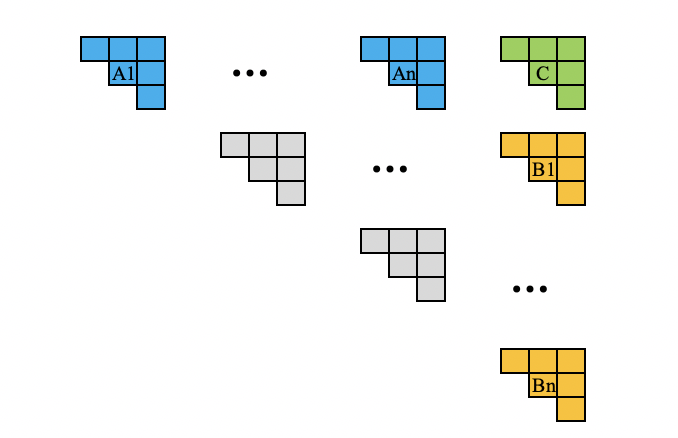
\includegraphics[scale=.74]{double_max_plus_dependence.png}}
\end{adjustbox}
\caption{Double max-plus dependency}
\label{fig:double_plus_dependencies}
\end{figure}
Thus, it can be $(j_{2}-i_{2}, i_{2}, k_{2})$ or $(i_{2}, j_{2}, k_{2})$ or $(M-i_{2}, j_{2}, k_{2})$ or $(i_{2}, j_{2}, k_{2})$ or $(j_{2}-i_{2}, k_{2}, i_{2})$ or $(-i_{2}$, $k_{2}$, $j_{2}$) etc.  However, auto-vectorization is prohibited if $k_{2}$ is the innermost loop iteration. 
\begin{figure}[htbp]
\begin{adjustbox}{varwidth=\textwidth,margin=0 {\abovecaptionskip} 0 0, frame=0.00pt}
\centerline{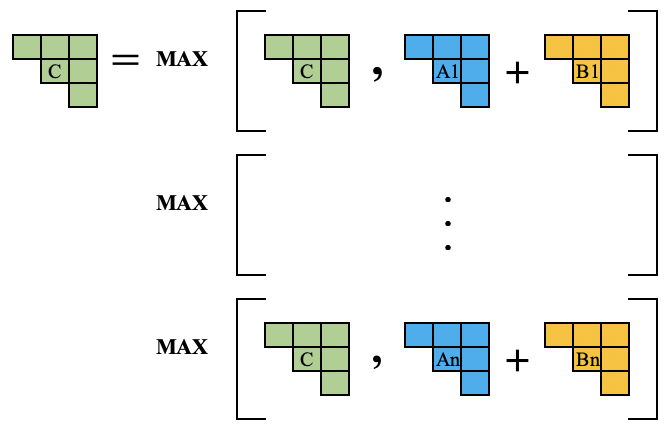
\includegraphics[scale=.74]{double_max_plus_accumulation_sequence.png}}
\end{adjustbox}
\caption{Double max-plus accumulation sequence}
\label{fig:double_max_plus_accumulation_sequence}
\end{figure}
Other choices can be viewed as loop permutations that allow auto-vectorization. For updating the final $F$-table entries, we can copy the data in any order. The original BPMax implementation uses $ i_{1},j_{1},i_{2},j_{2} \mapsto j_{1}-i_{1},j_{2}-i_{2},i_{1}, i_{2},k_{1},k_{2} $ schedule for double max-plus computation. 
Table~\ref{tab1:double_max_plus_schedule}  
shows various multi-dimensional affine schedules similar to Varadrajan’s. We pick similar schedules to establish the baseline since her kernel was based on multiply-add and ours is max-plus. Also, we use single-precision storage to reduce the memory footprint of BPMax.

\paragraph{Machine Peak Analysis and Micro-benchmark}
Next, we develop the roofline model for the target machine. Our schedule tries to exploit auto-vectorization that loads one scalar and vector of $8$ elements from L1 to compute $8$ max-plus operations, and the data access pattern is $ Y = \max (a+X, Y)$. We create a micro-benchmark to estimate the attainable L1 bandwidth for such access pattern. It allocates two large one-dimensional arrays for each thread, initializes them with random numbers, and
\begin{algorithm}
\caption{Max-plus streaming benchmark}
\label{algo:sequential_bench_mark}
\begin{algorithmic} [1]
  \FOR{$iteration \gets 0, MAX\_ITERATION$}
     \FOR{$index \gets 0, CHUNK\_SIZE$} 
     \STATE{$Y[index] = \max(alpha+X[index], Y[index])$} 
     \ENDFOR
  \ENDFOR 
\end{algorithmic}
\end{algorithm}
 then invokes the kernel (Algorithm~\ref{algo:sequential_bench_mark}) that computes the max-plus operation on the array.  The micro-benchmark data is presented in the result section.


\begin{table}[htbp]
\caption{\uppercase{Double max-plus schedule}}
\begin{center}
\begin{tabular}{|c|c|c|}
\hline
\textbf{} & \textbf{\textit{Variable}}& \textbf{\textit{Schedule}} \\
\hline
  & $F$ & $(i_{1},j_{1},i_{2},j_{2} \mapsto j_{1}-i_{1},i_{1},j_{1},i_{2},j_{2},j_{2})$   \\
\cline{2-3} 
$^{\mathrm{a}}$ & $R_{0}$ & $(i_{1},j_{1},i_{2},j_{2},k_{1},k_{2} \mapsto j_{1}-i_{1},i_{1},k_{1},i_{2},k_{2},j_{2})$,    \\
 & & $(i_{1},j_{1},i_{2},j_{2} \mapsto j_{1}-i_{1},i_{1},i_{1}-1,i_{2},i_{2}-1,j_{2})$ \\
\hline
  & $F$ & $(i_{1}, j_{1}, i_{2}, j_{2} \mapsto -i_{1}, j_{1}, j_{1}, -i_{2}, j_{2}, j_{2})$  \\
\cline{2-3} 
$^{\mathrm{b}}$ & $R_{0}$& $(i_{1},j_{1},i_{2},j_{2},k_{1},k_{2} \mapsto -i_{1},j_{1},k_{1},-i_{2},k_{2},j_{2})$ ,   \\
 & & $(i_{1},j_{1},i_{2},j_{2} \mapsto -i_{1},j_{1},i_{1}-1,-i_{2},i_{2}-1,j_{2})$ \\
\hline
  & $F$ & $(i_{1}, j_{1}, i_{2}, j_{2} \mapsto  j_{1}-i_{1}, i_{1}, j_{1}, i_{2}, j_{2}, j_{2})$   \\
\cline{2-3} 
$^{\mathrm{c}}$ & $R_{0}$& $(i_{1},j_{1},i_{2},j_{2},k_{1},k_{2} \mapsto j_{1}-i_{1},i_{1},k_{1},i_{2},k_{2},j_{2})$ ,   \\
 & & $(i_{1},j_{1},i_{2},j_{2} \mapsto j_{1}-i_{1},i_{1},i_{1}-1,i_{2},i_{2}-1,j_{2})$ \\
\hline
\multicolumn{3}{l}{$^{\mathrm{a}}$Fine-grain schedule(diagonal), parallel dimension 3}\\
\multicolumn{3}{l}{$^{\mathrm{b}}$Fine-grain schedule(bottom-up), parallel dimension 3}\\
\multicolumn{3}{l}{$^{\mathrm{c}}$Coarse-grain schedule, parallel dimension 1}
\end{tabular}
\label{tab1:double_max_plus_schedule}
\end{center}
\end{table}


\paragraph{Insights from Phase-I}
This phase highlights the possibility of further improvements of $R_{0}$ beyond loop permutation. Double max-plus performance attains just above  $20\%$ of our theoretical max-plus machine peak. We notice a significant collapse in performance when the input sequences are longer.
 
\subsection{Phase-II}
We have two objectives in this phase. First, find a complete schedule for BPMax that enables automatic vectorization for all the variables and estimate the other reduction term's overhead. Second, explore optimization opportunities for the double max-plus operation.
 
\paragraph{Multi-Dimensional Affine Schedule for BPMax}
Figure~\ref{fig:bpmax_dependency} shows the complete BPMax dependencies for a point. The point colored in red depends on all the other colored points.  BPMax has a total of five reductions. There are four additional reductions $R_{1}$ (green), $R_{2}$ (orange), $R_{3}$ (purple), $R_{4}$ (yellow) beside $R_{0}$ (blue). So, there are new dependencies in addition to the similar dependencies highlighted in the double max-plus computation. $R_{1}$ and $R_{2}$  have internal dependencies, but the other two have external dependencies. One common theme across various schedules is that $S^{(1)}$ and $S^{(2)}$ can be scheduled before scheduling any other variables. Also, order of filling up the inner triangle does not change with the introduction of the other terms. Thus, the first two dimensions of our multi-dimensional schedule can be either $(j_{1}-i_{1}, i_{1})$ or $(M-i_{1}, j_{1})$ or $(-i_{1}, j_{1})$ for $F$-table, $R_{0}$, $R_{1}$, $R_{2}$, $R_{3}$, $R_{4}$. $R_{3}$ and $R_{4}$ is over $k_{1}$ like $R_{0}$. So, the third dimension can be the same for all of them. Next, the inner three dimensions of the $R_{0}$ can also be the same as discussed earlier. $R_{3}$ and $R_{4}$  can use $(i_{2}, j_{2})$. However, we introduce additional terms to make the schedule dimension equal for all the variables. $F$-table, $R_{1}$, and $R_{2}$ must wait until $k_{1}$ reaches $j_{1}$ like double max-plus. 
\begin{figure}[htbp]
\begin{adjustbox}{varwidth=\textwidth,margin=0 {\abovecaptionskip} 0 0, frame=0.00pt}
\centerline{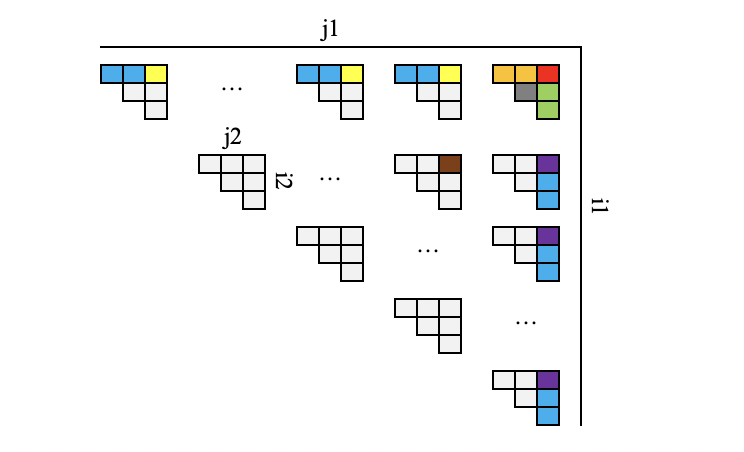
\includegraphics[scale=.66]{bpmax_dependency_new.png}}
\end{adjustbox}
\caption{BPMax dependency overview}
\label{fig:bpmax_dependency}
\end{figure}
 Thus, their third schedule dimension becomes $j_{1}$. Final $F$-table entries require intra-triangular dependencies to be evaluated which are similar to inter-triangular dependencies. So, it can be filled up diagonally or bottom-up and left to right.
\begin{table}[htbp]
\caption{\uppercase{BPMax fine-grain schedule}}
\begin{center}
\begin{tabular}{|c|c|}
\hline
\textbf{\textit{Variable}}& \textbf{\textit{Schedule}}$^{\mathrm{a}}$ \\
\hline
  $S^{(1)}, S^{(2)}$ & $(i_{1},j_{1} \mapsto 0, 0, 0, 0, j_{1}-i_{1}, i_{1}, 0, 0)$   \\
\cline{1-2} 
  $F$ & $(i_{1},j_{1},i_{2},j_{2} \mapsto 1, -i_{1}, j_{1}, j_{1}, -i_{2}, 0, j_{2},0)$   \\
\cline{1-2} 
$R_{1}, R_{2}$ & $(i_{1},j_{1},i_{2},j_{2},k_{2} \mapsto 1, -i_{1}, j_{1}, j_{1}, -i_{2}, 0, k_{2}, j_{2})$,    \\
 & $(i_{1},j_{1},i_{2},j_{2} \mapsto 1, -i_{1}, j_{1}, j_{1}, -i_{2}, 0, i_{2}-1, j_{2})$ \\
 \cline{1-2} 
 $R_{0}$ & $(i_{1},j_{1},i_{2},j_{2},k_{1},k_{2} \mapsto 1, -i_{1}, j_{1}, k_{1}, -1, -i_{2}, k_{2}, j_{2})$,    \\
  & $(i_{1},j_{1},i_{2},j_{2} \mapsto 1, -i_{1}, j_{1}, i_{1}-1, -1, -i_{2}, i_{2}-1, j_{2})$ \\
\cline{1-2} 
 $R_{3}, R_{4}$ & $(i_{1},j_{1},i_{2},j_{2},k_{1} \mapsto 1, -i_{1}, j_{1}, k_{1}, -1, -i_{2}, i2, j_{2})$,    \\
 & $(i_{1},j_{1},i_{2},j_{2} \mapsto 1, -i_{1}, j_{1}, i_{1}-1, -1, -i_{2}, i_{2}, j_{2})$ \\
 \cline{1-2} 
\hline
\multicolumn{2}{l}{$^{\mathrm{a}}$Parallel dimension 5}
\end{tabular}
\label{tab:bpm_fine_grain_schedule}
\end{center}
\end{table}
\begin{table}[htbp]
\caption{\uppercase{BPMax coarse-grain schedule}}
\begin{center}
\begin{tabular}{|c|c|}
\hline
\textbf{\textit{Variable}}& \textbf{\textit{Schedule}}$^{\mathrm{a}}$ \\
\hline
  $S^{(1)}, S^{(2)}$ & $(i_{1},j_{1} \mapsto 0, j_{1}-i_{1}, i_{1}, 0, 0, 0, 0)$   \\
\cline{1-2} 
  $F$ & $(i_{1},j_{1},i_{2},j_{2} \mapsto 1, j_{1}-i_{1}, i_{1}, j_{1}, -i_{2}, j_{2}, j_{2}$   \\
\cline{1-2} 
$R_{1}, R_{2}$ & $(i_{1},j_{1},i_{2},j_{2},k_{2} \mapsto 1, j_{1}-i_{1}, i_{1}, j_{1}, -i_{2}, k_{2}, j_{2})$ ,   \\
 & $(i_{1},j_{1},i_{2},j_{2} \mapsto 1, j_{1}-i_{1}, i_{1}, j1, -i_{2}, i_{2}-1, j_{2})$ \\
 \cline{1-2} 
$R_{0}$ & $(i_{1},j_{1},i_{2},j_{2},k_{1},k_{2} \mapsto 1, j_{1}-i_{1}, i_{1}, k_{1}, i_{2}, k_{2}, j_{2})$,    \\
 & $(i_{1},j_{1},i_{2},j_{2} \mapsto 1, j_{1}-i_{1}, i_{1}, i_{1}-1, i_{2}, i_{2}-1, j_{2})$ \\
\cline{1-2} 
$R_{3}, R_{4}$ & $(i_{1},j_{1},i_{2},j_{2},k_{1} \mapsto 1, j_{1}-i_{1}, i_{1}, k_{1}, i_{2}, i_{2}, j_{2})$,    \\
 & $(i_{1},j_{1},i_{2},j_{2} \mapsto 1, j_{1} -i_{1}, i_{1}, i_{1}-1, i_{2}, i_{2}, j_{2})$ \\
 \cline{1-2} 
\hline
\multicolumn{2}{l}{$^{\mathrm{a}}$Parallel Dimension 2}
\end{tabular}
\label{tab:bpm_coarse_grain_schedule}
\end{center}
\end{table}
Thus, the inner three dimensions of the schedule for $R_{1}$ and $R_{2}$ can be $(j_{2}-i_{2}, i_{2}, k_{2})$ or $(N-i_{2}, j_{2}, k_{2})$ or $(-i_{2}, j_{2}, k_{2})$ or $(j_{2}-i_{2}, k_{2}, j_{2})$ or $(N-i_{2}, k_{2}, j_{2})$ or $(-i_{2}, k_{2}, j_{2})$ etc. We carefully chose the schedule for $R_{1}$ and $R_{2}$ since the innermost $k_{2}$ prevents automatic vectorization.  We  ensure that $F$-table gets updated when $k_{2}$ reaches $j_{2}$. Table~\ref{tab:bpm_fine_grain_schedule} and ~\ref{tab:bpm_coarse_grain_schedule}  shows various multi-dimensional affine schedules which provide better results than the base schedule.  
 
\paragraph{Parallelization Approach} 
We take two different types of parallelization approach in this phase - coarse and fine-grain. For coarse-grain parallelization, threads work on distinct inner triangles simultaneously.  It is valid for $R_{0}$, $R_{1}$, $R_{2}$, $R_{3}$, and $R_{4}$. On the other hand, threads work on individual rows of an inner triangle simultaneously for fine-grain parallelization. It is only valid for $R_{0}$, $R_{3}$, and $R_{4}$. 



\paragraph{Memory Optimization} 
Memory-overhead of our \alphaz\ generated code is $M^2 \times N^2$. However, we only need one-fourth of that memory. Even though it seems inefficient, the unused elements are never moved between memory hierarchies. Reduction variables also take up memory space by default, which is wasteful. In this phase, coarse-grain parallelization still requires $P$ (number of threads) instances of a $2-D$ array for each reduction variables to be active in memory except $R_{0}$.
\begin{figure}[htbp]
\begin{adjustbox}{varwidth=\textwidth,margin=0 {\abovecaptionskip} 0 0, frame=0.00pt}
\centerline{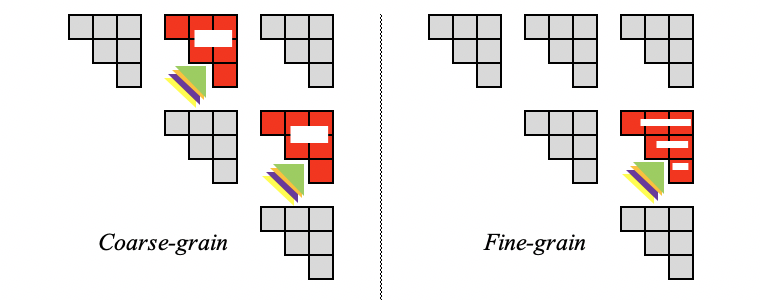
\includegraphics[scale=.585]{bpm_phase_2_memory_map.png}}
\end{adjustbox}
\caption{BPMax phase-II memory map}
\label{fig:bpm_phase_2_memory_map}
\end{figure}
$R_{0}$ shares memory with $F$. Fine-grain requires only a $2-D$ array for each of these variables illustrated in Figure~\ref{fig:bpm_phase_2_memory_map}.
 
\paragraph{Tiling $R_{0}$} 
The fine-grain parallelism for the $R_{0}$ assigns one or more rows to each thread. Processing each row needs to access one complete inner triangle below that row before moving to the next.  
\begin{figure}[htbp]
\begin{adjustbox}{varwidth=\textwidth,margin=0 {\abovecaptionskip} 0 0, frame=0.00pt}
\centerline{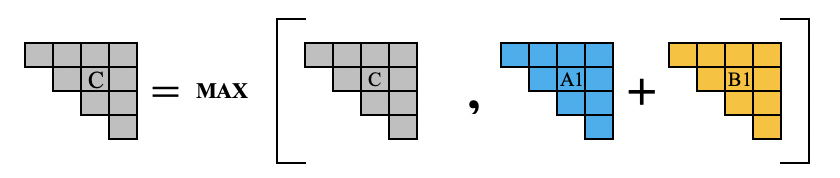
\includegraphics[scale=.57]{single_max_plus_operation.png}}
\end{adjustbox}
\caption{A matrix instance of max-plus operation}
\label{fig:matrix_instance_max_plus}
\end{figure}
It motivates us to tile computations of one matrix instance of max-plus operation. It is matrix multiplication like computation, except only a fraction of work is being done here, and the access pattern is imbalanced. We tile three inner dimensions with $k_{2}$ loop still in the middle and $j_{2}$ loop inside. So, this chops $(i_{2}, k_{2}, j_{2})$ iteration space, and we parallelize the outer $i_{2}$ dimension.

 \paragraph{Insights from Phase-II} 
Loop permutation and automatic vectorization provide a significant speedup for the entire BPMax program. However, the program suffers from imbalanced parallelization. The tiled version of the $R_{0}$ attains $33\%$ of our theoretical max-plus machine peak.

\subsection{Phase-III}
In this phase, we handle the load imbalance between threads and partially ($R_{0}$, $R_{3}$, $R_{4}$) apply tiling to BPMax.

\paragraph{Parallelization Approach}
Earlier, we have observed that the program quickly becomes DRAM-bound for the coarse-grain schedule since each thread computes an inner triangle. But, it allows us to parallelize $R_{1}$ and $R_{2}$.  On the other hand, $R_{0}$, $R_{3}$, and $R_{4}$ can be computed using the fine-grain schedule, which reduces data movement between DRAM and LLCs. However, $R_{1}$ and $R_{2}$ are not easy to parallelize.
\begin{table}[htbp]
\caption{\uppercase{BPMax hybrid schedule}}
\begin{center}
\begin{tabular}{|c|c|}
\hline
\textbf{\textit{Variable}}& \textbf{\textit{Schedule}}$^{\mathrm{a}}$ \\
\hline
 $S^{(1)}, S^{(2)}$ & $(i_{1},j_{1} \mapsto 0, 0, 0, j_{1}-i_{1}, i_{1}, 0, 0, 0)$   \\
\cline{1-2} 
 $F$ & $(i_{1},j_{1},i_{2},j_{2} \mapsto 1, j_{1}-i_{1}, M, 0, i_{1}, -i_{2}, j_{2}, 0$   \\
\cline{1-2} 
$R_{1}, R_{2}$ & $(i_{1},j_{1},i_{2},j_{2},k_{2} \mapsto 1, j_{1}-i_{1}, M, 0, i_{1}, -i_{2}, k_{2}, j_{2})$ ,   \\
 & $(i_{1},j_{1},i_{2},j_{2} \mapsto 1, j_{1}-i_{1}, M, 0, i_{1}, -i_{2}, i_{2}-1, j_{2})$ \\
 \cline{1-2} 
$R_{0}$ & $(i_{1},j_{1},i_{2},j_{2},k_{1},k_{2} \mapsto 1, j_{1}-i_{1}, i_{1}, k_{1}, i_{2}, k_{2}, j_{2}, 0)$,    \\
 & $(i_{1},j_{1},i_{2},j_{2} \mapsto 0, j_{1}-i_{1}, i_{1}, 0, i_{2}, 0, j_{2}, 0)$ \\
\cline{1-2} 
$R_{3}, R_{4}$ & $(i_{1},j_{1},i_{2},j_{2},k_{1} \mapsto 1, j_{1}-i_{1}, i_{1}, k_{1}, i_{2}, i_{2}, j_{2},0)$,    \\
 & $(i_{1},j_{1},i_{2},j_{2} \mapsto 0, j_{1}-i_{1}, i_{1}, 0, i_{2}, 0, j_{2}, 0)$ \\
 \cline{1-2} 
\hline
\multicolumn{2}{l}{$^{\mathrm{a}}$Parallel Dimension 4}
\end{tabular}
\label{tab:hybrid_schedule}
\end{center}
\end{table}
These are optimum string parenthesization (OSP)-like computations that require further transformation like middle serialization. If we use the fine-grain parallelism without such transformation, only one thread stays active, leading to lower CPU resource utilization. We take advantage of the best of both worlds. We use the fine-grain parallelism for $R_{0}$, $R_{3}$, $R_{4}$ and the coarse-grain parallelism for $F$-table, $R_{1}$, $R_{2}$. We call this hybrid schedule shown in Table ~\ref{tab:hybrid_schedule}. It improves CPU utilization and limits the data movement between DRAM and LLCs. However, there are some limitations discussed in the result section.


\paragraph{Tiling Integration and Subsystem Scheduling}
\alphaz\ produces inferior code when the tiling is applied to a subset of reduction operations. 
\begin{table}[htbp]
\caption{\uppercase{BPMax hybrid schedule with tiling}}
\begin{center}
\begin{tabular}{|c|c|c|}
\hline
\textbf{} & \textbf{\textit{Variable}}& \textbf{\textit{Schedule}} \\
\hline
 & ${\mathrm{c}}$& $(i_{1},j_{1} \mapsto M, i_{1}, j_{1}, 0)$ \\
 \cline{2-3} 
${\mathrm{a}}$ & $R_{0}$ & $(i_{1},j_{1},k_{1},k_{2} \mapsto k_{1}, i_{1}, k_{2}, j_{1})$,    \\
 & & $(i_{1},j_{1} \mapsto -1, i_{1}, 0, j_{1})$ \\
\cline{2-3} 
& $R_{3}, R_{4}$ & $(i_{1},j_{1},k_{1} \mapsto k_{1}, i_{1}, i_{1}, j_{1})$,    \\
 & & $(i_{1},j_{1} \mapsto -1, i_{1}, 0, j_{1})$ \\
 \cline{2-3} 
\hline
& $S^{(1)}, S^{(2)}$ & $(i_{1},j_{1} \mapsto 0, 0, j_{1}-i_{1}, i_{1}, 0, 0, 0)$   \\
\cline{2-3} 
& ${\mathrm{d}}$ & $(i_{1},j_{1} \mapsto 1, j_{1}-i_{1}, i_{1}, j_{1}-4, 0, 0, 0)$   \\
\cline{2-3} 
${\mathrm{b}}$ & $F$ & $(i_{1},j_{1},i_{2},j_{2} \mapsto 1, j_{1}-i_{1}, M, i_{1}, -i_{2}, j_{2}, 0)$   \\
\cline{2-3} 
& $R_{1}, R_{2}$ & $(i_{1},j_{1},i_{2},j_{2},k_{2} \mapsto 1, j_{1}-i_{1}, M, i_{1}, -i_{2}, k_{2}, j_{2})$ ,   \\
 & & $(i_{1},j_{1},i_{2},j_{2} \mapsto 1, j_{1}-i_{1}, M, i_{1}, -i_{2}, i_{2}-1, j_{2})$ \\
\hline
\multicolumn{3}{l}{}\\
\multicolumn{3}{l}{${\mathrm{a}}$ - Subsystem schedule(parallel dimension 1)}\\
\multicolumn{3}{l}{${\mathrm{b}}$ - Root system schedule(parallel dimension 3)}\\
\multicolumn{3}{l}{${\mathrm{c}}$ - Subsystem output}\\
\multicolumn{3}{l}{${\mathrm{d}}$ - Subsystem call}\\
\end{tabular}
\label{tab:hybrid_schedule_with_tiling}
\end{center}
\end{table}
It is due to the insertion of additional schedule dimensions needed to isolate the tiling band. So, we use \alfa\ subsystem, which partitions BPMax computation into two systems. The subsystem produces an inner triangle using $R_{0}$, $R_{3}$, $R_{4}$ and the primary system produces $R_{1}$ and $R_{2}$ along with final $F$-table output and consolidates the results from the subsystem. It allows us to modularize the program and apply tiling transformation on $R_{0}$, $R_{3}$, and $R_{4}$ efficiently. The subsystem gets called for each instance of an inner $F$-table update.  Finally, \textit{use equation} construct integrates these two systems. We invoke the subsystem call for each instance of the iteration space defined by the schedule's first two dimensions. Now, this requires us to specify the schedule for the subsystem invocation. Both systems are integrated manually. We perform minimal preprocessing since our code generator can not produce tiled code for the subsystem automatically. Two lines of source code changes are made to achieve this. Table~\ref{tab:hybrid_schedule_with_tiling} summarizes the complete schedule for the two systems.

 
\paragraph{Memory Optimization}
We further optimize memory utilization in this phase. $R_{0}$, $R_{3}$ and $R_{4}$ are always computed before final $F$-table update. So, they share the memory with $F$-table. 
\begin{figure}[htbp]
\begin{adjustbox}{varwidth=\textwidth,margin=0 {\abovecaptionskip} 0 0, frame=0.00pt}
\centerline{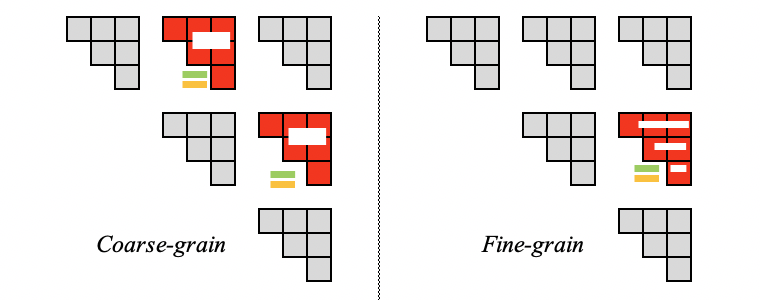
\includegraphics[scale=.63]{bpm_phase_3_memory_map.png}}
\end{adjustbox}
\caption{BPMax phase-III memory map}
\label{fig:bpm_phase_3_memory_map}
\end{figure}
Also, only one row of an inner triangle is required for $R_{1}$ and $R_{2}$ to keep up with the $F$-table update. This has been highlighted in Figure ~\ref{fig:bpm_phase_3_memory_map}. We also optimize redundant data copies during subsystem call using \textit{setMemorySpaceForUseEquationOptimization} transformation. 

\paragraph{Performance Tuning}
To find an optimum tile shape, we start with cubic tiles and then adjust one or more dimensions to find a better tile shape that works moderately well across various inputs. However,  we notice 10\% performance differences between the best and generic tile sizes. 
\begin{figure}[htbp]
\begin{adjustbox}{varwidth=\textwidth,margin=0 {\abovecaptionskip} 0 0, frame=0.00pt}
\centerline{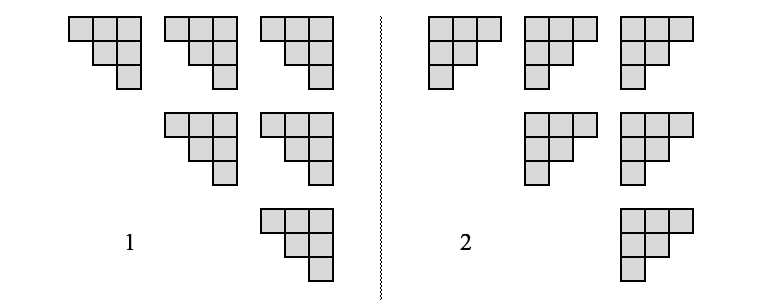
\includegraphics[scale=.63]{memory_map_update.png}}
\end{adjustbox}
\caption{Memory mapping schemes}
\label{fig:memory_map_schemes}
\end{figure}
The OMP dynamic-schedule works better than the static and guided-schedule due to an imbalanced workload. Next, we perform some manual memory optimization. The schedule initializes memory for each reduction body. Still, when one variable shares memory space with multiple variables,  memory initialization becomes redundant, and the current code generator does not optimize it. We comment out these macros, which attempt duplicate initializations to eliminate redundancies. We have tried two different memory transformations for the inner triangle highlighted in  Figure~\ref{fig:memory_map_schemes} - 1 : $(i_{2}, j_{2} \mapsto i_{2}, j_{2})$   and 2 : $(i_{2}, j_{2} \mapsto i_{2}, j_{2}-i_{2})$. Option-1 always performs better.

%\paragraph{Validation of Program Correctness}
%In addition to checking the final scores between reference and optimized version, 
%We use \alphaz\ toolset to verify the correctness of the optimized program using a verifier that compares outputs of a schedule code with sequential code. However, this is not sufficient due to max-plus operation.  We develop a parallel version of the BPMax program to replace the max-plus operation with plus-plus operation and apply the exact same sequence of transformations and ran it through the verifier to ensure that our transformations and schedules do not change the semantics of the original program. %One of the major challenge was to run the validation on longer sequences since the base and sequential implementations are extremely slow. 

%\paragraph{Validation of Program Correctness}
%In addition to checking the final scores between reference and optimized version, We use \alphaz\ toolset to verify the correctness of the optimized program using a verifier that compares outputs of a schedule code with the sequential code. %However, this is not sufficient due to max-plus operation.  We develop a parallel version of the BPMax program to replace the max-plus operation with plus-plus operation and apply the exact same sequence of transformations and ran it through the verifier to ensure that our transformations and schedules do not change the semantics of the original program. %One of the major challenge was to run the validation on longer sequences since the base and sequential implementations are extremely slow.
